\chapter{2}{Vektorer i planet och rummet}
\begin{task}{2.1 a)}
	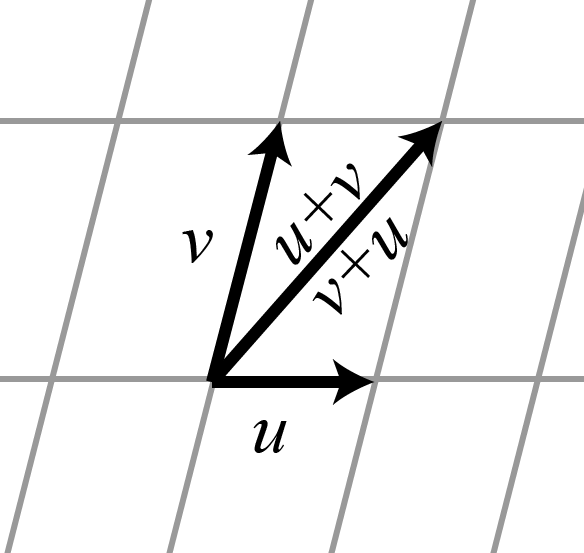
\includegraphics[scale=0.2]{images/21a.PNG}
\end{task}

\begin{task}{b)}
	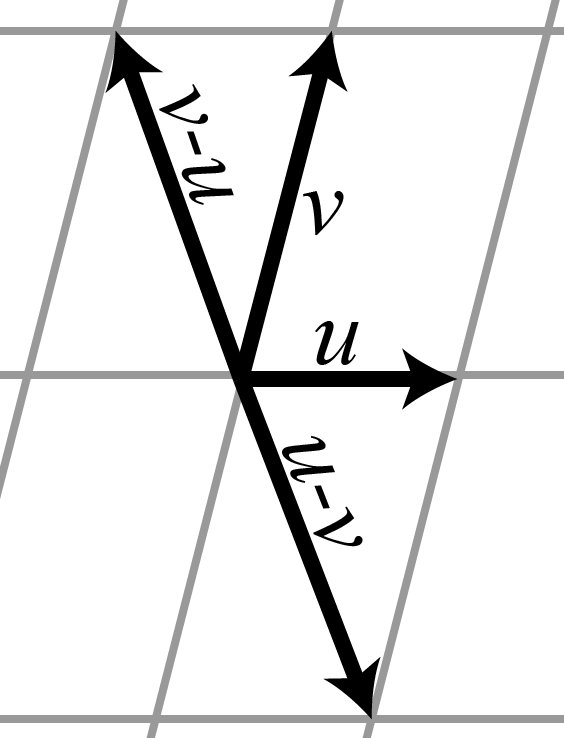
\includegraphics[scale=0.2]{images/21b.PNG}
\end{task}

\begin{task}{c)}
	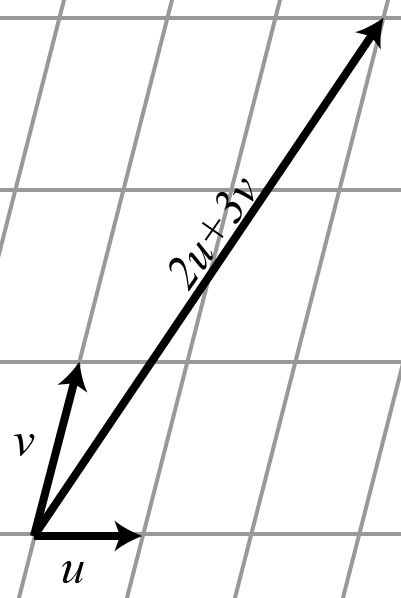
\includegraphics[scale=0.3]{images/21c.PNG}
\end{task}

\begin{task}{d)}
	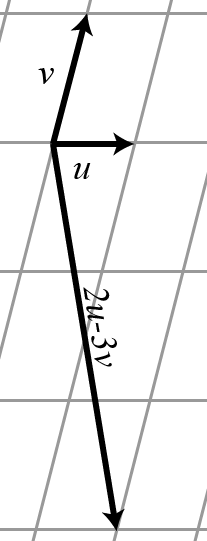
\includegraphics[scale=0.3]{images/21d.PNG}
\end{task}

\begin{task}{2.2}
	\ans Nollvektor
\end{task}

\pagebreak
\begin{task}{2.3}
	Gausselimination:
	\begin{align*}
		&\begin{linsys}{rrr}
			 \hat{u}+& \hat{v}=&u \\
			2\hat{u}+&3\hat{v}=&u
		\end{linsys}
		&\begin{array}{l}
			(a) \\
			(b)
		\end{array} \\ \lra
		&\begin{linsys}{rrr}
			\hat{u}+&\hat{v}=&u \\
			        &\hat{v}=&v-2u
		\end{linsys}
		&\begin{array}{l}
		(a')=(a) \\
		(b')=(b)-2(a)
		\end{array} \\ \lra
		&\begin{cases}
		\hat{v}=v-2u \\
		\hat{u}=u-(v-2u)=3u-v
		\end{cases}
	\end{align*}
	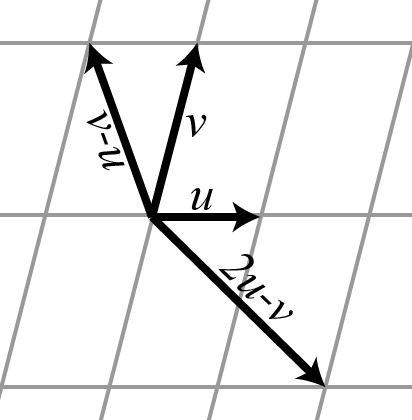
\includegraphics[scale=0.3]{images/23.PNG}
	
	\ans $\hat{v}=v-2u$, $\hat{u}=3u-v$
\end{task}

\begin{task}{2.4}
	\[\vek{OC}=\vek{OA}+\vek{AC}=\vek{OA}+\frac{1}{4}\vek{AB}\]
	\[\vek{OA}=\vek{OB}-\vek{AB} \lra
	\vek{AB}=\vek{OB}-\vek{OA}\]
	\[\vek{OC}=
	\vek{OA}+\frac{1}{4}\vek{AB}=
	\vek{OA}+\frac{1}{4}(\vek{OB}-\vek{OA})=
	\frac{3}{4}\vek{OA}+\frac{1}{4}\vek{OB} \mproof\]
\end{task}

\begin{task}{2.5}
	\[\vek{OM}=\vek{OB}-\vek{MB}=\vek{OB}-\frac{1}{2}\vek{AB}\]
	\[\vek{OB}-\vek{AB}=\vek{OA} \lra
	\vek{AB}=\vek{OB}-\vek{OA}\]
	\[\vek{OM}=
	\vek{OB}-\frac{1}{2}\vek{AB}=
	\vek{OB}-\frac{1}{2}(\vek{OB}-\vek{OA})=
	\frac{1}{2}(\vek{OB}+\vek{OA}) \mproof\]
\end{task}

\begin{task}{2.6}
	Enligt uppgiften:
	\[\vek{AM}=\frac{2}{3}\vek{AA_1}\]
	Vilket ger:
	\[\vek{OM}=
	\vek{OA}+\vek{AM}=
	\vek{OA}+\frac{2}{3}\vek{AA_1}\]
	Mittpunktsformeln:
	\[\vek{AA_1}=\frac{1}{2}(\vek{AB}+\vek{AC})\]
	Vilket ger:
	\[\vek{OM}=
	\vek{OA}+\frac{2}{3}\*\frac{1}{2}(\vek{AB}+\vek{AC})=
	\vek{OA}+\frac{1}{3}(\vek{AB}+\vek{AC})\]
	Enligt figuren:
	\[\vek{AB}=\vek{OB}-\vek{OA},~~
	\vek{AC}=\vek{OC}-\vek{OA}\]
	Vilket ger:
	\[\vek{OM}=
	\vek{OA}+\frac{1}{3}(\vek{OB}-\vek{OA}+\vek{OC}-\vek{OA})=
	\frac{1}{3}(\vek{OA}+\vek{OB}+\vek{OC}) \mproof\]
\end{task}

\begin{task}{2.7}
	Enligt uppgiften:
	\[\vek{AM}=\frac{3}{4}\vek{AA_1}\]
	Vilket ger:
	\[\vek{OM}=
	\vek{OA}+\vek{AM}=
	\vek{OA}+\frac{3}{4}\vek{AA_1}\]
	Tyngdpunktsformeln:
	\[\vek{AA_1}=\frac{1}{3}(\vek{AB}+\vek{AC}+\vek{AD})\]
	Vilket ger:
	\[\vek{OM}=
	\vek{OA}+\frac{3}{4}\*\frac{1}{3}(\vek{AB}+\vek{AC}+\vek{AD})=
	\vek{OA}+\frac{1}{4}(\vek{AB}+\vek{AC}+\vek{AD})\]
	Enligt figuren:
	\[\vek{AB}=\vek{OB}-\vek{OA},~~
	\vek{AC}=\vek{OC}-\vek{OA},~~
	\vek{AD}=\vek{OD}-\vek{OA}\]
	Vilket ger:
	\[\vek{OM}=
	\vek{OA}+\frac{1}{4}(\vek{OB}-\vek{OA}+\vek{OC}-\vek{OA}+\vek{OD}-\vek{OA})=
	\frac{1}{4}(\vek{OA}+\vek{OB}+\vek{OC}+\vek{OD}) \text{~~~~V.S.V}\]
\end{task}

\begin{task}{2.8}
	Låt $O$ ligga i punkten $M$. tyngdpunktsformeln ger:
	\[\vek{OM}=\frac{1}{3}(\vek{OA}+\vek{OB}+\vek{OC})\]
	Eftersom $O=M$:
	\[\begin{cases}
	\vek{OM}=0 \\
	\vek{OA}=\vek{MA} \\
	\vek{OB}=\vek{MB} \\
	\vek{OC}=\vek{MC}
	\end{cases}\]
	Vilket ger:
	\[\frac{1}{3}(\vek{MA}+\vek{MB}+\vek{MC})=0 \lra
	\vek{MA}+\vek{MB}+\vek{MC}=3\*0=0 \text{~~~~V.S.V}\]
\end{task}

\begin{task}{2.9}
	Låt $O$ vara en godtycklig punkt i rummet. Vilket ger:
	\[\begin{cases}
	\vek{A_1A_2}=\vek{OA_2}-\vek{OA_1} \\
	\vek{B_1B_2}=\vek{OB_2}-\vek{OB_1} \\
	\vek{C_1C_2}=\vek{OC_2}-\vek{OC_1}
	\end{cases}\]
	Tyngdpunktsformeln baklänges samt hur differens för vektorer funkar ger:
	\begin{align*}
	&\vek{A_1A_2}+\vek{B_1B_2}+\vek{C_1C_2}=
	\vek{OA_2}-\vek{OA_1}+\vek{OB_2}-\vek{OB_1}+\vek{OC_2}-\vek{OC_1}= \\ =
	&3\*\frac{1}{3}(\vek{OA_2}+\vek{OB_2}+\vek{OC_2})-3\*\frac{1}{3}(\vek{OA_1}+\vek{OB_1}+\vek{OC_1})= \\ =
	&3(\vek{OM_2}-\vek{OM_1})=
	3\vek{M_1M_2} \text{~~~~V.S.V}
	\end{align*}
\end{task}

\begin{task}{2.10}
	Mittpunktsformeln ger:
	\[\begin{cases}
	\vek{OA_m}=\frac{1}{2}(\vek{OA}+\vek{OB}) \\
	\vek{OB_m}=\frac{1}{2}(\vek{OB}+\vek{OC}) \\
	\vek{OC_m}=\frac{1}{2}(\vek{OC}+\vek{OA})
	\end{cases}\]
	Vilket ger:
	\begin{align*}
	&VL=\vek{OA_m}+\vek{OB_m}+\vek{OC_m}=
	\frac{1}{2}(\vek{OA}+\vek{OB})+\frac{1}{2}(\vek{OB}+\vek{OC})+\frac{1}{2}(\vek{OC}+\vek{OA})= \\ =
	&\frac{1}{2}(2\vek{OA}+2\vek{OB}+2\vek{OC})=
	\vek{OA}+\vek{OB}+\vek{OC}=HL \text{~~~~V.S.V}
	\end{align*}
\end{task}

\begin{task}{2.11}
	Låt $ABCD$ vara en godtycklig tetraeder i rummet och $O$ vara en godtycklig punkt i rummet. 
	Om alla sammanbindningar skär tyngdpunkt vet vi även att alla skär varandra i tyngdpunkten.
	Antag att tyngdpunkten ligger i punkten $M$ och $\vek{OM}=\frac{1}{4}(\vek{OA}+\vek{OB}+\vek{OC}+\vek{OD})$.

	Mittpunktsformeln ger:
	\[\begin{array}{lcr}
	p_1=\frac{1}{2}(\vek{OA}+\vek{OB}) & \text{~~~~motsatta punkt:~~~~} & q_1=\frac{1}{2}(\vek{OC}+\vek{OD}) \\
	p_2=\frac{1}{2}(\vek{OB}+\vek{OC}) & \text{~~~~motsatta punkt:~~~~} & q_2=\frac{1}{2}(\vek{OA}+\vek{OD}) \\
	p_3=\frac{1}{2}(\vek{OC}+\vek{OA}) & \text{~~~~motsatta punkt:~~~~} & q_3=\frac{1}{2}(\vek{OB}+\vek{OD})
	\end{array}\]
	En slumpmässig punkt på varje sammanbindning kan beskrivas som där $x,y,z$ ligger mellan 0 och 1:
	\[\begin{array}{l}
	s_1=p_1+x(q_1-p_1)=\frac{1}{2}(\vek{OA}+\vek{OB})+x\frac{1}{2}((\vek{OA}+\vek{OB})-(\vek{OC}+\vek{OD})) \\
	s_2=p_2+y(q_2-p_2)=\frac{1}{2}(\vek{OB}+\vek{OC})+y\frac{1}{2}((\vek{OB}+\vek{OC})-(\vek{OA}+\vek{OD})) \\
	s_2=p_3+z(q_3-p_3)=\frac{1}{2}(\vek{OC}+\vek{OA})+z\frac{1}{2}((\vek{OC}+\vek{OA})-(\vek{OB}+\vek{OD}))
	\end{array}\]
	Om vi sätter $x=y=z=\frac{1}{2}$ så kommer $s_1=s_2=s_3=\frac{1}{4}(\vek{OA}+\vek{OB}+\vek{OC}+\vek{OD})$ vilket är samma punkt som vi antog att tyngdpunkten $M$ skulle ligga i. Eftersom alla tre skär $M$ skär även alla tre varandra i $M$. ~~V.S.V
\end{task}

\begin{task}{2.12}
	Låt $O$ vara en godtycklig punkt i rummet. 
	Om två stycken sträckor beskriver samma vektor måste de vara parallella enligt definitionen från vektorer. 
	Så om $\vek{A_1B_1}=\vek{D_1C_1}$ och $\vek{B_1C_1}=\vek{A_1D_1}$ är $A_1B_1C_1D_1$ en parallellogram.

	mittpunktsformeln:
	\[\begin{array}{l}
	\vek{OA_1}=\frac{1}{2}(\vek{OA}+\vek{OB}) \\
	\vek{OB_1}=\frac{1}{2}(\vek{OB}+\vek{OC}) \\
	\vek{OC_1}=\frac{1}{2}(\vek{OC}+\vek{OD}) \\
	\vek{OD_1}=\frac{1}{2}(\vek{OD}+\vek{OA})
	\end{array}\]
	\[\begin{array}{l}
	\vek{A_1B_1}=\vek{OB_1}-\vek{OA_1}=\frac{1}{2}(\vek{OB}+\vek{OC}-(\vek{OA}+\vek{OB}))=\frac{1}{2}(\vek{OC}-\vek{OA}) \\
	\vek{D_1C_1}=\vek{OC_1}-\vek{OD_1}=\frac{1}{2}(\vek{OC}+\vek{OD}-(\vek{OD}+\vek{OA}))=\frac{1}{2}(\vek{OC}-\vek{OA}) \\
	\vek{B_1C_1}=\vek{OC_1}-\vek{OB_1}=\frac{1}{2}(\vek{OC}+\vek{OD}-(\vek{OB}+\vek{OC}))=\frac{1}{2}(\vek{OD}-\vek{OB}) \\
	\vek{A_1D_1}=\vek{OD_1}-\vek{OA_1}=\frac{1}{2}(\vek{OD}+\vek{OA}-(\vek{OA}+\vek{OB}))=\frac{1}{2}(\vek{OD}-\vek{OB})
	\end{array}\]
	$\vek{A_1B_1}=\vek{D_1C_1}$ och $\vek{B_1C_1}=\vek{A_1D_1}$ är alltså sant vilket innebär att $A_1B_1C_1D_1$ är en parallellogram. ~~V.S.V
\end{task}

\pagebreak
\begin{task}{2.13 a)}
	\[u_1=3e_1+2e_2\]
	
	\ans $(3,2)$
\end{task}

\begin{task}{b)}
	\[u_2=2e_1+3e_2\]
	
	\ans $(2,3)$
\end{task}

\begin{task}{c)}
	\[u_3=-2e_1+2e_2\]
	
	\ans $(-2,2)$
\end{task}

\begin{task}{d)}
	\[u_4=-3e_1-2e_2\]
	
	\ans $(-3,-2)$
\end{task}

\begin{task}{e)}
	\[u_5=2e_1-3e_2\]
	
	\ans $(2,-3)$
\end{task}

\begin{task}{f)}
	\[e_1=1e_1+0e_2\]
	
	\ans $(1,0)$
\end{task}

\begin{task}{g)}
	\[e_2=0e_1+1e_2\]
	
	\ans $(0,1)$
\end{task}

\begin{task}{2.14 a)}
	$\hat{v}=v-2u$, $\hat{u}=3u-v$
	\begin{align*}
		&u=a\hat{u}+b\hat{v}=
		a(3u-v)+b(v-2u)=
		(3a-2b)u+(b-a)v \lra \\ \lra
		&\begin{cases}
			3a-2b=1 \\
			b-a=0
		\end{cases} \lra
		\begin{cases}
			a=1 \\ 
			b=1
		\end{cases} \lra
		u=1\hat{u}+1\hat{v}
	\end{align*}
	
	\begin{align*}
		&u=a\hat{u}+b\hat{v}=
		a(3u-v)+b(v-2u)=
		(3a-2b)u+(b-a)v \lra \\ \lra
		&\begin{cases}
			3a-2b=0 \\
			b-a=1
		\end{cases} \lra
		\begin{cases}
			a=2 \\ 
			b=3
		\end{cases} \lra
		u=2\hat{u}+3\hat{v}
	\end{align*}
	
	\ans $u:~(1,1)$ och $v:~(2,3)$
\end{task}

\begin{task}{b)}
	\[\hat{u}=3u-v=3u-1v\]
	\[\hat{v}=v-2u=-2u+1v\]
	
	\ans $\hat{u}:~(3,-1)$ och $\hat{v}:~(-2,1)$
\end{task}

\begin{task}{2.15}
	\[\vek{OC}=\frac{3}{4}\vek{OA}+\frac{1}{4}\vek{OB}\]
	
	\ans $\vek{OC}:~(3/4,1/4)$
\end{task}

\begin{task}{2.16}
	För $\vek{TC}$ använd tyndpunktsformeln och låt $T$ vara den godtyckliga punkten i rummet.
	\[\vek{TT}=\frac{1}{3}(\vek{TA}+\vek{TB}+\vek{TC}) \lra
	0=\frac{1}{3}\vek{TA}+\frac{1}{3}\vek{TB}+\frac{1}{3}\vek{TC} \lra
	\vek{TC}=-\vek{TA}-\vek{TB}\]
	För $\vek{TM}$ använd mittpunktsformeln där $T$ är den godtyckliga punkten i rummet.
	\[\vek{TM}=\frac{1}{2}(\vek{TA}+\vek{TB})=\frac{1}{2}\vek{TA}+\frac{1}{2}\vek{TB}\]
	
	\ans $\vek{TC}:~(-1,-1)$ och $\vek{TM}:~(1/2,1/2)$
\end{task}

\begin{task}{2.17 a)}
	Vi ansätter lösningen:
	\[(4,1,-5)=x(2,1,-1)+y(1,1,1)\]
	Identifierar variablerna (gausselimination):
	\[\begin{cases}
		2x+y=4 \\
		x+y=1 \\
		-x+y=-5
	\end{cases} \lra
	\begin{cases}
		2x+y=4 \\
		y=-2 \\
		3y=-6
	\end{cases} \lra
	\begin{cases}
		x=3 \\
		y=-2
	\end{cases}\]
	
	\ans $(4,1,-5)$ är en linjärkombination av $u_1$ och$u_2$
\end{task}

\begin{task}{b)}
	Vi ansätter lösningen:
	\[(4,3,2)=x(2,1,-1)+y(1,1,1)\]
	Identifierar variablerna (gausselimination):
	\[\begin{cases}
		2x+y=4 \\
		x+y=3 \\
		-x+y=2
	\end{cases} \lra
	\begin{cases}
		2x+y=4 \\
		y=2 \\
		3y=0
	\end{cases} \lra
	y=2\neq0 \ra \text{ Saknar lösning.}\]
	
	\ans $(4,3,2)$ är inte en linjärkombination av $u_1$ och$u_2$
\end{task}

\begin{task}{c)}
	Vi ansätter lösningen:
	\[(-9,-7,-3)=x(2,1,-1)+y(1,1,1)\]
	Identifierar variablerna (gausselimination):
	\[\begin{cases}
		2x+y=-9 \\
		x+y=-7 \\
		-x+y=-3
	\end{cases} \lra
	\begin{cases}
		2x+y=-9 \\
		y=-5 \\
		3y=-15
	\end{cases} \lra
	\begin{cases}
		x=-7 \\
		y=-5
	\end{cases}\]
	
	\ans $(-9,-7,-3)$ är en linjärkombination av $u_1$ och$u_2$
\end{task}

\begin{task}{2.18 a)}
	För att två vektorer ska vara parallella ska det finnas ett $k$ så att:
	\[u=kv\]
	Ansätt därför en lösning och identifiera $k$ och $a$:
	\[(a,1+a)=k(2,-3) \lra
	\begin{cases}
		a=2k \\
		1+a=-3k
	\end{cases} \lra
	\begin{cases}
		a=-\frac{2}{5} \\
		k=-\frac{1}{5}
	\end{cases}\]
	
	\ans $a=-\frac{2}{5}$
\end{task}

\begin{task}{b)}
	För att två vektorer ska vara parallella ska det finnas ett $k$ så att:
	\[u=kv\]
	Ansätt därför en lösning och identifiera $k$ och $a$:
	\[(a,-3)=k(2,1-a) \lra
	\begin{cases}
		a=2k \\
		-3=k(1-a)
	\end{cases}\]
	Substitutionsmetoden:
	\[-3=k(1-2k) \lra
	2k^2-k-3=0 \lra
	k^2-\frac{k}{2}-\frac{3}{2}=0\]
	\[k=\frac{1}{4}\pm\sqrt{\frac{1}{16}+\frac{24}{16}}=\frac{1}{4}\pm\frac{5}{4}\]
	\[\begin{cases}
		k_1=\frac{3}{2} \lra a_1=3 \\
		k_2=-1 \lra a_2=-2
	\end{cases}\]
	
	\ans $a=3$ eller $a=-2$
\end{task}

\begin{task}{c)}
	För att två vektorer ska vara parallella ska det finnas ett $k$ så att:
	\[u=kv\]
	Ansätt därför en lösning och identifiera $k$ och $a$:
	\[(a,3)=k(2,1-a) \lra
	\begin{cases}
		a=2k \\
		3=k(1-a)
	\end{cases}\]
	Substitutionsmetoden:
	\[3=k(1-2k) \lra
	2k^2-k+3=0 \lra
	k^2-\frac{k}{2}+\frac{3}{2}=0\]
	\[k=\frac{1}{4}\pm\sqrt{\frac{1}{16}-\frac{24}{16}}=\frac{1}{4}\pm\sqrt{-\frac{23}{16}} \ra \text{ Saknar reell lösning}\]

	\ans Saknar lösning
\end{task}

\begin{task}{d)}
	För att två vektorer ska vara parallella ska det finnas ett $k$ så att:
	\[u=kv\]
	Ansätt därför en lösning och identifiera $k$ och $a$:
	\[(a,1+a,3)=k(4,2,-6) \lra
	\begin{cases}
		a=4k \\
		1+a=2k \\
		3=-6k
	\end{cases} \lra
	\begin{cases}
		a=4k \\
		1=-2k \\
		3=-6k
	\end{cases} \lra
	\begin{cases}
		a=-2 \\
		k=-\frac{1}{2}
	\end{cases}\]
	
	\ans $a=-2$
\end{task}

\begin{task}{2.19 a)}
	För att vektorerna ska vara linjärt beroende ska de gå att beskriva med hjälp av varandra vilket innebär att det ska finnas ett $k$ så att:
	\[(2,4)=k(-4,-2)\]
	Identifiera variabeln:
	\[\begin{cases}
		2=-4k \\
		4=-2k
	\end{cases} \lra
	k=-\frac{1}{2}\neq-2 \ra \text{ saknar lösning}\]
	
	\ans Vektorerna är inte linjärt beroende
\end{task}

\begin{task}{b)}
	För att vektorerna ska vara linjärt beroende ska de gå att beskriva med hjälp av varandra vilket innebär att det ska finnas ett $k$ så att:
	\[(6,-3)=k(-4,2)\]
	Identifiera variabeln:
	\[\begin{cases}
		6=-4k \\
		-3=2k
	\end{cases} \lra
	k=-\frac{3}{2}\]
	
	\ans Vektorerna är linjärt beroende
\end{task}

\begin{task}{c)}
	För att vektorerna ska vara linjärt beroende ska de vara parallella och enligt definition är nollvektorn $(0,0)$ parallell med alla vektorer och därför är vektorerna linjärt beroende.
	
	\ans Vektorerna är linjärt beroende
\end{task}

\begin{task}{d)}
	För att vektorerna ska vara linjärt beroende ska de gå att beskriva med hjälp av varandra vilket innebär att det ska finnas ett $k_1$ och ett $k_2$ så att:
	\[(1,0)=k_1(0,1)+k_2(7,5)\]
	Identifiera variablerna:
	\[\begin{cases}
		1=7k_2 \\
		0=k_1+5k_2
	\end{cases} \lra
	\begin{cases}
		k_1=-\frac{5}{7} \\
		k_2=\frac{1}{7}
	\end{cases} \ra \text{ linjärt beroende}\]
	
	\ans Vektorerna är linjärt beroende
\end{task}

\begin{task}{e)}
	För att vektorerna ska vara linjärt beroende ska de gå att beskriva med hjälp av varandra vilket innebär att det ska finnas ett $k_1$ och ett $k_2$ så att:
	\[(5,9)=k_1(3,-2)+k_2(2,1)\]
	Identifiera variablerna:
	\[\begin{cases}
		5=3k_1+2k_2 \\
		9=-2k_1+k_2
	\end{cases} \lra
	\begin{cases}
		k_1=-\frac{13}{7} \\
		k_2=\frac{37}{7}
	\end{cases} \ra \text{ linjärt beroende}\]
	
	\ans Vektorerna är linjärt beroende
\end{task}

\begin{task}{2.20 a)}
	För att vektorerna ska vara linjärt beroende ska de gå att beskriva med hjälp av varandra vilket innebär att det ska finnas ett $k_1$ och ett $k_2$ så att:
	\[(1,1,1)=k_1(3,1,2)+k_2(0,2,1)\]
	Identifiera variablerna:
	\[\begin{cases}
		1=3k_1+0k_2 \\
		1=k_1+2k_2 \\
		1=2k_1+k_2
	\end{cases} \lra
	\begin{cases}
		k_1=\frac{1}{3} \\
		k_2=\frac{1}{3}
	\end{cases} \ra \text{ linjärt beroende}\]
	
	\ans Vektorerna är linjärt beroende
\end{task}

\begin{task}{b)}
	För att vektorerna ska vara linjärt beroende ska de gå att beskriva med hjälp av varandra vilket innebär att det ska finnas ett $k_1$ och ett $k_2$ så att:
	\[(0,1,1)=k_1(1,0,1)+k_2(1,1,0)\]
	Identifiera variablerna:
	\[\begin{cases}
		0=k_1+k_2 \\
		1=0k_1+k_2 \\
		1=k_1+0k_2
	\end{cases} \lra
	\begin{cases}
		k_1=1 \\
		k_2=1\neq-1
	\end{cases} \ra \text{ linjärt oberoende}\]
	
	\ans Vektorerna är inte linjärt beroende
\end{task}

\begin{task}{c)}
	För att vektorerna ska vara linjärt beroende ska de gå att beskriva med hjälp av varandra vilket innebär att det ska finnas ett $k$ så att:
	\[(1,1,1)=k(3,1,2)\]
	Identifiera variabeln:
	\[\begin{cases}
		1=3k \\
		1=k \\
		1=2k
	\end{cases} \lra
	k=\frac{1}{3}\neq1\neq\frac{1}{2} \ra \text{ linjärt oberoende}\]
	
	\ans Vektorerna är inte linjärt beroende
\end{task}

\begin{task}{d)}
	För att vektorerna ska vara linjärt beroende ska de gå att beskriva med hjälp av varandra vilket innebär att det ska finnas ett $k$ så att:
	\[(1,0,2)=k(-2,0,-4)\]
	Identifiera variabeln:
	\[\begin{cases}
		1=-2k \\
		0=0k \\
		2=-4k
	\end{cases} \lra
	k=-\frac{1}{2} \ra \text{ linjärt beroende}\]
	
	\ans Vektorerna är linjärt beroende
\end{task}

\begin{task}{e)}
	Eftersom $(1,0,2)$ och $(-2,0,-4)$ är linjärt beroende (se \taskref{d)}) är även $(2,0,3)$, $(1,0,2)$ och $(-2,0,-4)$ det.
	
	\ans Vektorerna är linjärt beroende
\end{task}

\begin{task}{f)}
	För att vektorerna ska vara linjärt beroende ska de gå att beskriva med hjälp av varandra vilket innebär att det ska finnas ett $k_1$ och ett $k_2$ så att:
	\[(1,0,2)=k_1(3,0,4)+k_2(5,0,6)\]
	Identifiera variablerna (gausselimination):
	\[\begin{cases}
		1=3k_1+5k_2 \\
		0=0k_1+0k_2 \\
		2=4k_1+6k_2
	\end{cases} \lra
	\begin{cases}
		k_1=2 \\
		k_2=-1
	\end{cases}\ra \text{ linjärt beroende}\]
	
	\ans Vektorerna är linjärt beroende
\end{task}

\begin{task}{g)}
	För att vektorerna ska vara linjärt beroende ska de gå att beskriva med hjälp av varandra vilket innebär att det ska finnas ett $k_1$, ett $k_2$ och ett $k_3$ så att:
	\[(1,1,0)=k_1(1,0,1)+k_2(0,1,1)+k_3(3,3,3)\]
	Identifiera variablerna (gausselimination):
	\[\begin{cases}
		1=k_1+0k_2+3k_3 \\
		1=0k_1+k_2+3k_3 \\
		0=k_1+k_2+3k_3
	\end{cases} \lra
	\begin{cases}
		k_1=-1 \\
		k_2=-1 \\
		k_3=\frac{2}{3}
	\end{cases}\ra \text{ linjärt beroende}\]
	
	\ans Vektorerna är linjärt beroende
\end{task}

\begin{task}{2.21}
	För att vektorerna ska vara linjärt beroende ska de gå att beskriva med hjälp av varandra (de ska vara parallella) vilket innebär att det ska finnas ett $k$ och $a$ så att:
	\[(a,-2)=k(1,a-1)\]
	Identifiera variabeln:
	\[\begin{cases}
		a=k \\
		-2=k(a-1)
	\end{cases}\]
	Substitutionsmetoden:
	\[-2=k(k-1) \lra
	k^2-k+2=0\]
	\[k=\frac{1}{2}\pm\sqrt{\frac{1}{4}-\frac{8}{4}}=\frac{1}{2}\pm\sqrt{-\frac{7}{4}} \ra \text{ saknar reell lösning}\]
	
	\ans Nej, det finns inget $a$ så att vektorerna är linjärt beroende
\end{task}

\begin{task}{2.22 a)}
	\[u=5e_1+3e_2\]
	
	\ans $(5,3)$
\end{task}

\begin{task}{b)}
	Ja, eftersom de inte är parallella.
	
	\ans Ja
\end{task}

\begin{task}{c)}
	\[2\hat{e}_1+\hat{e}_2=u\]

	\ans $(2,1)$
\end{task}

\begin{task}{d)}
	\[\hat{e}_1=e_1+2e_2 \ra (1,2)\]
	\[\hat{e}_2=3e_1-e_2 \ra (3,-1)\]
	
	\ans $\hat{e}_1:~(1,2)$ och $\hat{e}_2:~(3,-1)$
\end{task}

\begin{task}{e)}
	\begin{align*}
		&x_1e_1+x_2e_2=v=
		\hat{x}_1\hat{e}_1+\hat{x}_2\hat{e}_2=
		\hat{x}_1(e_1+2e_2)+\hat{x}_2(3e_1-e_2)= \\ =
		&(\hat{x}_1+3\hat{x}_2)e_1+(2\hat{x}_1-\hat{x}_2)e_2 \ra (x_1,x_2)=(\hat{x}_1+3\hat{x}_2,2\hat{x}_1-\hat{x}_2)
	\end{align*}
\end{task}

\begin{task}{2.23}
	$\hat{e}_1$ och $\hat{e}_2$ kan användas som bas om de inte är parallella så genom att anta att de är parallella kan vi bestämma om de kan användas som bas eller inte. De är parallella om det finns ett $k$ så att:
	\[\hat{e}_1=k\hat{e}_2\] 
	\[\hat{e}_1=k\hat{e}_2 \lra
	-e_1+2e_2=k(3e_1+4e_2) \lra
	\begin{cases}
		-1=3k \\
		2=4k
	\end{cases} \lra
	k=-\frac{1}{3}\neq\frac{1}{2}\]
	Linjerna är inte parallella och därför kan de vara en bas i planet.
	\begin{align*}
		&\begin{cases}
			\hat{e}_1=-e_1+2e_2 \\
			\hat{e}_2=3e_1+4e_2
		\end{cases} \lra
		\begin{cases}
			e_1=-\hat{e}_1+2e_2 \\
			e_2=\frac{1}{4}\hat{e}_2-\frac{3}{4}e_1
		\end{cases}\lra \\ \lra
		&\begin{cases}
			e_1=-\hat{e}_1+2(\frac{1}{4}\hat{e}_2-\frac{3}{4}e_1) \\
			e_2=\frac{1}{4}\hat{e}_2-\frac{3}{4}(-\hat{e}_1+2e_2)
		\end{cases}\lra
		\begin{cases}
			e_1=-\frac{2}{5}\hat{e}_1+\frac{1}{5}\hat{e}_2 \\
			e_2=\frac{3}{10}\hat{e}_1+\frac{1}{10}\hat{e}_2
		\end{cases}
	\end{align*}
	Sätt sedan in i uttrycket för vektorn.
	\begin{align*}
		&u=4e_1-5e_2=
		4(-\frac{2}{5}\hat{e}_1+\frac{1}{5}\hat{e}_2)-5(\frac{3}{10}\hat{e}_1+\frac{1}{10}\hat{e}_2)= \\ =
		&-\frac{8}{5}\hat{e}_1-\frac{15}{10}\hat{e}_1+\frac{4}{5}\hat{e}_2-\frac{5}{10}\hat{e}_2=
		-\frac{31}{10}\hat{e}_1+\frac{3}{10}\hat{e}_2
	\end{align*}
	
	\ans $(-3.1,0.3)$
\end{task}

\pagebreak
\begin{task}{2.24 a)}
	För att visa att $e^{'}_1$, $e^{'}_2$ och $e^{'}_3$ är en bas i rummet behöver vi först visa att  $e^{'}_1$ och $e^{'}_2$ är linjärt oberoende i planet och sedan visa att $e^{'}_3$ är linjärt oberoende i rummet.
	
	Om det inte finns $k$ så att:
	\[e^{'}_1=ke^{'}_2\]
	är $e^{'}_1$ och $e^{'}_2$ linjärt oberoende i planet.
	\begin{align*}
		&e^{'}_1=ke^{'}_2 \lra
		e^1+0e^2+0e^3=k(2e^1+e^2+0e^3) \lra \\ \lra
		&\begin{cases}
			1=2k \\
			0=k \\
			0=0
		\end{cases} \lra
		k=\frac{1}{2}\neq0 \lra
		\text{ linjärt oberoende}
	\end{align*}
	Om det inte finns $k_1$ och $k_2$ så att:
	\[e^{'}_3=k_1e^{'}_1+k_2e^{'}_2\]
	är $e^{'}_1$, $e^{'}_2$ och $e^{'}_3$ linjärt oberoende i rummet.
	\begin{align*}
		&e^{'}_3=k_1e^{'}_1+k_2e^{'}_2 \lra \\ \lra
		&3e^1+2e^2+e^3=k_1(e^1+0e^2+0e^3)+k_2(2e^1+e^2+0e^3) \lra \\ \lra
		&\begin{cases}
			3=k_1+2k_2 \\
			2=k_2 \\
			1\neq0
		\end{cases} \lra
		1\neq0 \lra
		\text{ linjärt oberoende}
	\end{align*}
	\ans $e^{'}_1$, $e^{'}_2$ och $e^{'}_3$ är en bas i rummet.
\end{task}

\begin{task}{b)}
	\[x^{'}_1e^{'}_1+x^{'}_2e^{'}_2+x^{'}_3e^{'}_3=x_1e_1+x_2e_2+x_3e_3\]
	\begin{align*}
		VL=&x^{'}_1(e_1)+x^{'}_2(2e_1+e_2)+x^{'}_3(3e_1+2e_2+e_3)= \\ =
		&(x^{'}_1+2x^{'}_2+3x^{'}_3)e_1+(x^{'}_2+2x^{'}_3)e_2+x^{'}_3e_3
	\end{align*}
	identifiera variablerna:
	\[\begin{cases}
		x_1=x^{'}_1+2x^{'}_2+3x^{'}_3 \\
		x_2=x^{'}_2+2x^{'}_3 \\
		x_3=x^{'}_3
	\end{cases}\]
\end{task}

\begin{task}{c)}
	\[u=
	2e_1+7e_3 \lra
	\begin{cases}
		2=x^{'}_1+2x^{'}_2+3x^{'}_3 \\
		0=x^{'}_2+2x^{'}_3 \\
		7=x^{'}_3
	\end{cases} \lra
	\begin{cases}
		x^{'}_3=7 \\
		x^{'}_2=-14 \\
		x^{'}_1=9
	\end{cases}\]
	
	\ans $(x^{'}_1,x^{'}_2,x^{'}_3)=(9,-14,7)$
\end{task}

\pagebreak
\begin{task}{2.25}
	Visa att $\hat{e}_1$, $\hat{e}_2$ och $\hat{e}_3$ är linjärt oberoende.
	\begin{align*}
		&\lambda_1\hat{e}_1+\lambda_2\hat{e}_2+\lambda_3\hat{e}_3=0 \lra \\ \lra
		&\lambda_1(e_1+e_2)+\lambda_2(e_1+e_2-e_3)+\lambda_3(e_2-e_3)=0 \lra \\ \lra
		&(\lambda_1+\lambda_2)e_1+(\lambda_1+\lambda_2+\lambda_3)e_2+(-\lambda_2-\lambda_3)e_3=0 \lra \\ \lra
		&\begin{cases}
		0=\lambda_1+\lambda_2 \\
		0=\lambda_1+\lambda_2+\lambda_3 \\
		0=-\lambda_2-\lambda_3 \\
	\end{cases}
	\end{align*}
	Enda lösningen är $\lambda_1=\lambda_2=\lambda_3=0$ vilket innebär att de är linjärt oberoende och där med en möjlig bas i rummet.
	\[u=2e_1+3e_2-2e_3=\hat{x}_1\hat{e}_1+\hat{x}_2\hat{e}_2+\hat{x}_3\hat{e}_3\]
	\begin{align*}
		HL=&\hat{x}_1(e_1+e_2)+\hat{x}_2(e_1+e_2-e_3)+\hat{x}_3(e_2-e_3)= \\ =
		&(\hat{x}_1+\hat{x}_2)e^1+(\hat{x}_1+\hat{x}_2+\hat{x}_3)e^2+(-\hat{x}_2-\hat{x}_3)e^3
	\end{align*}
	Identifiera variablerna (gausselimination):
	\[\begin{cases}
		2=\hat{x}_1+\hat{x}_2 \\
		3=\hat{x}_1+\hat{x}_2+\hat{x}_3 \\
		-2=-\hat{x}_2-\hat{x}_3
	\end{cases} \lra
	\begin{cases}
		2=\hat{x}_1+\hat{x}_2 \\
		1=\hat{x}_3 \\
		-2=-\hat{x}_2-\hat{x}_3
	\end{cases} \lra
	\begin{cases}
		\hat{x}_3=1 \\
		\hat{x}_2=1 \\
		\hat{x}_1=1
	\end{cases}
	\]
	
	\ans $(1,1,1)$
\end{task}

\begin{task}{2.26}
	\ans
\end{task}

\begin{task}{2.27}
	\ans
\end{task}

\begin{task}{2.28 a)}
	\ans
\end{task}

\begin{task}{b)}
	\ans
\end{task}

\begin{task}{2.29}
	\ans
\end{task}

\begin{task}{2.30}
	\ans
\end{task}